\documentclass[spanish]{udpreport}
\usepackage[utf8]{inputenc}
\usepackage[spanish]{babel}
\graphicspath{{images/}}
\usepackage{graphicx}
\usepackage{multirow}
\usepackage{verbatim} 
\usepackage{upgreek} 

% Podemos establecer el logo de alguna entidad o dejar el de la UDP (defecto)
\setlogo{EITFI}

\title{Metodologia RUP}
\author{Christian López \\ Thomas Muñoz \\ Flavio Pallini}
\email{christian.lopeza@mail.udp.cl \\ thomas.munoz@mail.udp.cl \\ flavio.pallini@mail.udp.cl}
\date{29 de agosto de 2017}

% Además podemos establecer la facultad y escuela
% los valores por defecto son los siguientes:
\udpschool{Escuela de Informática y Telecomunicaciones}
\udpfaculty{Facultad de Ingeniería y Ciencias}
\udpuniversity{Universidad Diego Portales}

\begin{document}
\maketitle

\tableofcontents
\listoffigures

\chapter{Introducción}
Según la IEEE, "la ingeniería de software es la aplicación de un enfoque sistemático, disciplinado y cuantificable al desarrollo, operación, y mantenimiento del software." Bajo este concepto, si bien es posible construir software sin seguir un protocolo para la planificación de su desarrollo, resulta mucho más conveniente y seguro utilizar alguna metodología aplicada de la ingeniería como pauta a seguir, a fin de modelar la solución a un problema en una empresa que pueda ser resuelto con la implementación o mejora de un nuevo software. De esta forma se gestionan múltiples variables y procesos esperados de forma más eficiente y con un riesgo de error menor. \par
Por lo general, las metodologías de trabajo se basan en un conocimiento de las necesidades a suplir por el proyecto, la determinación de su alcance, su construcción, y su evaluación como respuesta al problema original. Dependiendo de la metodología usada, estas etapas pueden sucederse de forma lineal, cíclica, en ese mismo o distinto orden, dependiendo de lo que el proyecto amerite. Así, en este informe, se detallará la metodología RUP, o \textit{Rational Unified Process}.
% Hoy en día es casi imposible realizar un proyecto de software sin hacer uso de alguna metodología, ya que estos requieren de un manejo de muchas variables, métodos y procesos. Es por esto que para satisfacer estas necesidades se hace uso de la ingeniería de software como pauta a seguir cuando se quiere modelar la solución a un problema de software en una empresa.\par

\chapter{Explicación de Metodología}
La metodología RUP es un proceso de desarrollo de software creado por \textit{Rational Software}, y actualmente propiedad de IBM. Es una de las metodologías de desarrollo de software más utilizadas para el análisis, implementación y documentación de sistemas orientados a objetos. Se caracteriza por no ser estática, sino compuesta por un conjunto de fases adaptables según la necesidad del cliente o avance del equipo de desarrollo.\par
Esta metodología trabaja con iteraciones, haciendo a RUP una forma de desarrollo en espiral. Cada iteración incluye los roles que se van a ver involucrados, las labores que se van a realizar, y el subproducto que van a producir. Sin embargo, estas iteraciones se diseñan tal que puedan dividir el proceso de desarrollo en cuatro grandes fases, donde cada una incluye en mayor o menor medida el modelamiento del negocio, análisis, diseño, construcción, pruebas e implantación. Lo que esto permite es un desarrollo maleable donde nuevos desafíos o requerimientos pueden ser adheridos al proyecto, y donde el producto final necesariamente debe haber sido compuesto por, y probado como, componentes interdependientes, lo cual permite probar más de cerca la calidad del código.

\section{¿Por qué utilizar RUP?}
\label{sec: Por que utilizar RUP}
RUP proporciona información sobre lo que puede esperarse de la tarea de desarrollo. Ofrece un glosario de terminología y una enciclopedia de conocimiento que le ayuda a comunicar sus necesidades de forma eficaz al equipo de  desarrollo de software. \par
Para un gestor o jefe de equipo, RUP proporciona  un proceso el cual le permite comunicarse de forma eficaz con el personal, gestionar la planificación y el control de su trabajo. Para un Diseñador, RUP proporciona una buena base de arquitectura y una gran cantidad de materiales con las que construir una definición de un proceso, lo que le permite configurar y ampliar dicha base como desee.

\section{¿Cuándo debo utilizar RUP?}
\label{sec: Cuando debo utilizar RUP}
Se utiliza RUP desde el inicio de  un proyecto de software, y puede seguir utilizándolo en los ciclos de desarrollo subsiguientes tiempo después de que le proyecto inicial haya terminado. \par
La forma de utilizar RUP varía para ajustarse a sus necesidades. Existen unas pocas consideraciones que determinarán cuando y como utilizar partes diferentes de RUP.
\begin{itemize}
\item Ciclo vital del proyecto(numero de iteraciones, longitud de cada fase)
\item Propósitos empresariales, visión, ámbito y riesgo del proyecto
\item Tamaño del esfuerzo de desarrollo de software
\end{itemize}
En la siguiente figura \ref{fig:grafico} muestra a través de un gráfico de complejidad de técnica y gestión:

\begin{figure}[h]
	\centering
	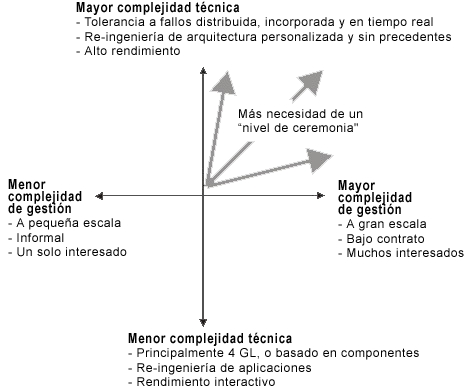
\includegraphics[width=0.7\textwidth]{RUP.png}
	\caption{\label{fig:grafico}Gráfico complejidad de técnica y gestión.}
\end{figure}

\section{Fases de la metodología RUP}
Las fases indican el énfasis que se da en el proyecto en un instante dado. Para capturar la dimensión temporal de un proyecto, RUP divide el proyecto en cuatro fases diferentes(ver figura \ref{fig:fases}):

\begin{figure}[!h]
	\centering
	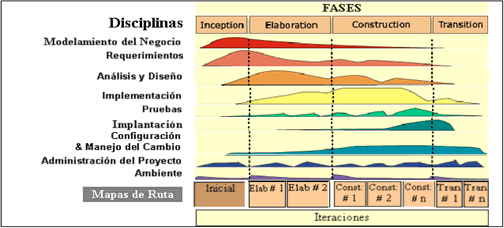
\includegraphics[width=0.8\textwidth]{fases.png}
	\caption{\label{fig:fases}Fases de RUP.}
\end{figure}

\begin{itemize}
\item Iniciación o Diseño: énfasis en el alcance del sistema
\item Preparación: énfasis en la arquitectura
\item Construcción: énfasis en el desarrollo
\item Transición: énfasis en la aplicación

\end{itemize}

\subsection{Fase de Inicio}
\label{subsec:inicio}
El objetivo preferente de esta fase es alcanzar un acuerdo entre todos los interesados respecto a los objetivos del ciclo vital del proyecto.
Es muy significativa la fase de inicio, pues son más arriesgados para los requisitos y para la actividad comercial y deben abordarse antes de que el proyecto pueda continuar.\par
La duracion de esto es generalmente corto y se utiliza para definir si es factible seguir y definir los riesgos. Un prototipo se puede hacer para que el cliente pruebe el software.\par


\subsection{Fase de elaboracion}
\label{subsec:elaboracion}
El proposito de esta fase es el establecimiento de una arquitectura de sistema para proporcionar una base estable para el diseño y la implementación en la fase de construccion. La arquitetura va evolucionando  a partir de una consideracion de requisitos mas significativos y  una valoracion a los riesgos.\par
Al final de la fase de elaboración se encuentra el segundo objectivo mas importante del proyecto que es el ciclo vital de la arquitectura. En esta se examina los objectivos y el ámbito del sistema detallado, la eleccion de arquitectura y la resolucion a los principales riesgos.

\subsection{Fase de Construcción}
\label{subsec:construccion}
El objectivo de la fase de construccion es aclarar lo requisitos restantes y completar el desarrolo del sistema basandose en la base de la arquitectura.
En esta fase sespone el énfasis en la gestion de los recursos y el control de la operaciones para poder optimizar los costes, la planificacion y la calidad.\par

\subsection{Fase de Transición}
En esta fase se garantiza que el software este diponible para los usuarios finales, ademas se puede acarrear varias iteraciones e incluye las pruebas del producto en preparación para el release, asi como los ajustes menores basados en la informacion obtenida de los usuarios que han probado el software.\par
En este momento del ciclo vital, la informacion recibida de los usuarios debe centrarse especialmente en el ajuste del producto, las cuestiones de configuracion, instalacion y utilización.

\section{Desventajas de RUP}
Siendo una metodología iterativa donde cada iteración tiene un grado significativo de independencia, las principales desventajas de RUP tienen que ver con la integración de todas las iteraciones en un proyecto coherente. En particular, se debe poner atención especial en compatibilizar los procesos y tecnologías de cada componente entre sí. Asimismo, si bien es conveniente evaluar la calidad de los componentes por separado, no se puede obviar el control de calidad del producto completo, gracias al problema de compatibilización ya mencionado.
Dependiendo de la granularidad de las iteraciones contra el alcance del proyecto, trabajar con RUP puede ser más desorganizado que otras metodologías. Si bien son claras las fases de RUP y éstas otorgan un nivel de orden, existen varios proyectos que no se pueden subdividir tan óptimamente. Similarmente, esto puede llevar a una construcción más difícil que con otras metodologías.
Finalmente, y como detalle final, dividir el trabajo de esta forma puede complejizar la documentación.

\chapter{Aplicación en Canchapp}

\chapter{Conclusión}


%\listoftables


\end{document}

